% id: 108-e12
% book: 개념원리 기하 · 13 정사영
% section: 필수·발전 예제
% figure: crop:fig-108-e12.png
% answer: ⑴ $4$ ⑵ $\dfrac{\sqrt{2}}{4}$
% answer_source: 본문 풀이
% variant_level: 0 (원본 전사)
% 이 파일은 build.mjs 가 items.json 에서 만든다. 고칠 때는 items.json 을 고친다.
\smash{\raisebox{1.5mm}{\dmkichul{개념원리 기하 108쪽 예제 12 · 필수}}}
\noindent\begin{minipage}[t]{0.58\linewidth}\vspace{0pt}\raggedright 오른쪽 그림과 같이 밑면이 정사각형이고 옆면이 모두 합동인 이등변삼각형으로 이루어진 사각뿔에서 다음을 구하시오.\end{minipage}\hfill\begin{minipage}[t]{0.4\linewidth}\vspace{0pt}\centering \setlength{\dmfigw}{89.0pt}\ifdim\dmfigw>\linewidth\setlength{\dmfigw}{\linewidth}\fi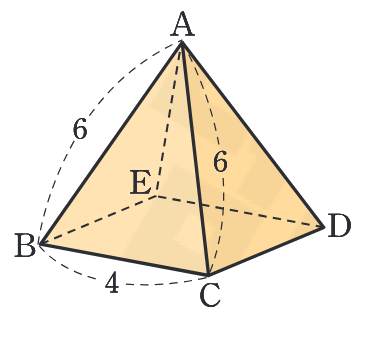
\includegraphics[width=\dmfigw]{figures/fig-108-e12.png}\end{minipage}\par
\dmsubprob{1} 삼각형~$\pt{ABC}$의 평면~$\pt{BCDE}$ 위로의 정사영의 넓이
\dmsubprob{2} 평면~$\pt{ABC}$와 평면~$\pt{BCDE}$가 이루는 각의 크기를 $\theta$라 할 때, $\cos\theta$의 값
